\section{The Model \label{model}}
%\subsection{Automatic discovery of a factorised latent space}

We wish to relate two views $Y \in \mathbb{R}^{N\times D_Y}$ and
$Z\in\mathbb{R}^{N\times D_Z}$ of a dataset within the same model. We
assume the existence of a single latent variable $X\in
\mathbb{R}^{N\times Q}$ which, through the mappings
$\{f^Y_d\}_{d=1}^{D_Y}: X \mapsto Y$ and $\{f^Z_d\}_{d=1}^{D_Z}: X
\mapsto Z$ ($Q<D$), gives a low dimensional representation of the
data. Our assumption is that the data is generated from a low
dimensional manifold and corrupted by additive Gaussian noise
$\epsilon^{\{Y,Z\}} \sim \mathcal{N}(\bfz, \sigma^{\{Y,Z\}}_{\epsilon} I)$,
%$\epsilon$
\begin{align}
  y_{nd} &= f^Y_d(\mathbf{x}_n) + \epsilon^Y_{nd}\nonumber\\
  z_{nd} &= f^Z_d(\mathbf{x}_n) + \epsilon^Z_{nd},
\end{align}
where $\{y,z\}_{nd}$ represents dimension $d$ of point $n$.  This
leads to the likelihood under the model, $P(Y,Z|X,\bftheta)$, where
$\bftheta = \{\bftheta^Y, \bftheta^Z\}$ collectively denotes the 
%parameters of the mappings.  
parameters of the mapping functions and the noise variances $\sigma_{\epsilon}^{\{Y,Z\}}$.
Finding the latent representation $X$ and the mappings
$f^Y$ and $f^Z$ is an ill-constrained problem. \citet{Lawrence:2005vk}
suggested regularizing the problem by placing Gaussian process (GP)
\cite{Rasmussen:book06} priors over the mappings and the resulting models
are known as Gaussian Process latent variable models (GP-LVMs).

In the GP-LVM framework each generative mapping is modeled as a
product of independent GP's parametrized by a (typically shared)
covariance function $k^{\{Y,Z\}}$ evaluated over the latent variable
$X$, so that
\begin{equation}
\label{pfx}
p(F^Y|X, \bftheta^Y) = \prod_{d=1}^{D_Y} \mathcal{N}(\bff^Y_d | \bfz, K^Y) ,
\end{equation}
where $F^Y = \{\bff^Y_d\}_{d=1}^{D_Y}$ with $f^Y_{nd} = f^Y_d(\bfx_n)$, and
similarly for $F^Z$.
%% :
%% \begin{equation}
%% \label{eq:GPpriors}
%%  f^{\{Y,Z\}}_d(\bfx)  \sim \mathcal{GP}\left(0, k^{\{Y,Z\}}(\bfx_i, \bfx_j) \right),
%%  %f^Z_d(\bfx) & \sim \mathcal{GP}\left(0, k^Z(\bfx_i, \bfx_j) \right)
%% \end{equation}
%% where the covariance functions $k^Y$ and $k^Z$ define the properties of the mappings.
This allows for general non-linear mappings to be marginalised out
analytically leading to a likelihood as a product of Gaussian
densities,
\begin{equation}
\resizebox{.9\hsize}{!}{$P(Y,Z | X,\bftheta) = 
  \prod_{\mathcal{K} = \{Y,Z\}} \int p(\mathcal{K} | F^\mathcal{K})
   p(F^\mathcal{K} | X, \bftheta^\mathcal{K}) \intd F^\mathcal{K}.$} \label{eq:likelihood}
    %& \int p(Y | F^Y) p(F^Y | X, \bftheta^Y) \intd F^Y \cdot \nonumber \\
	%&\int p(Z | F^Z) p(F^Z | X, \bftheta^Z) \intd F^Z. \label{eq:likelihood}
\end{equation}
%
%\begin{align}
%P(Y,Z|X,\bftheta) = 
%\prod_{n=1}^N \Big( 
%    & \int p(\bfy_n|\bfx_n, \bftheta^Y) \intd f^Y \cdot \nonumber \\
%	& \int p(\bfzi_n|\bfx_n, \bftheta^Z) \intd f^Z \Big). \label{eq:likelihood}
%\end{align}
%
A fully Bayesian treatment requires integration over the latent
variable $X$ in equation \eqref{eq:likelihood} which is intractable,
as $X$ appears non-linearly in the inverse of the covariance matrices
$K^Y$ and $K^Z$ of the GP priors for $f^Y$ and $f^Z$. In practice, a
maximum a posteriori solution
\cite{Shon:2006wr,Ek:2007uo,Salzmann:2010vh} was often used. However,
failure to marginalize out the latent variables means that it is not
possible to automatically estimate the dimensionality of the latent space or the
parameters of any prior distributions used in the latent space. We
show how we can obtain an approximate Bayesian training and inference
procedure by variationally marginalizing out $X$. 
%This allows us to
%estimate the latent space's dimensionality and the prior distributions over
%the latent variables. 
We achieve this by building on recent
variational approximations for standard GP-LVMs
\cite{Titsias:bayesGPLVM10,Damianou:vgpds11}. We then introduce
\emph{automatic relevance determination} (ARD) priors
\cite{Rasmussen:book06} so that each view of the data is allowed to estimate
a separate vector of ARD parameters. This allows the views to determine
which of the emerging private and shared latent spaces are relevant to
them. We refer to this idea as \emph{manifold relevance determination}
(MRD).% to be used for the mappings.  This is central
% to our model as it allows each dimension to be associated with a
% weight which defines its ``importance'' with respect to reconstructing
% the observed data. In \cite{Titsias:bayesGPLVM10} this was used as a
% means of learning the dimensionality of the latent space directly from
% data while here we additionally exploit this to learn a factorization
% of the latent variable.

\subsection{Manifold Relevance Determination}
% Force figure to be come a page earlier
%
\begin{figure*}[t]
  \begin{center}
    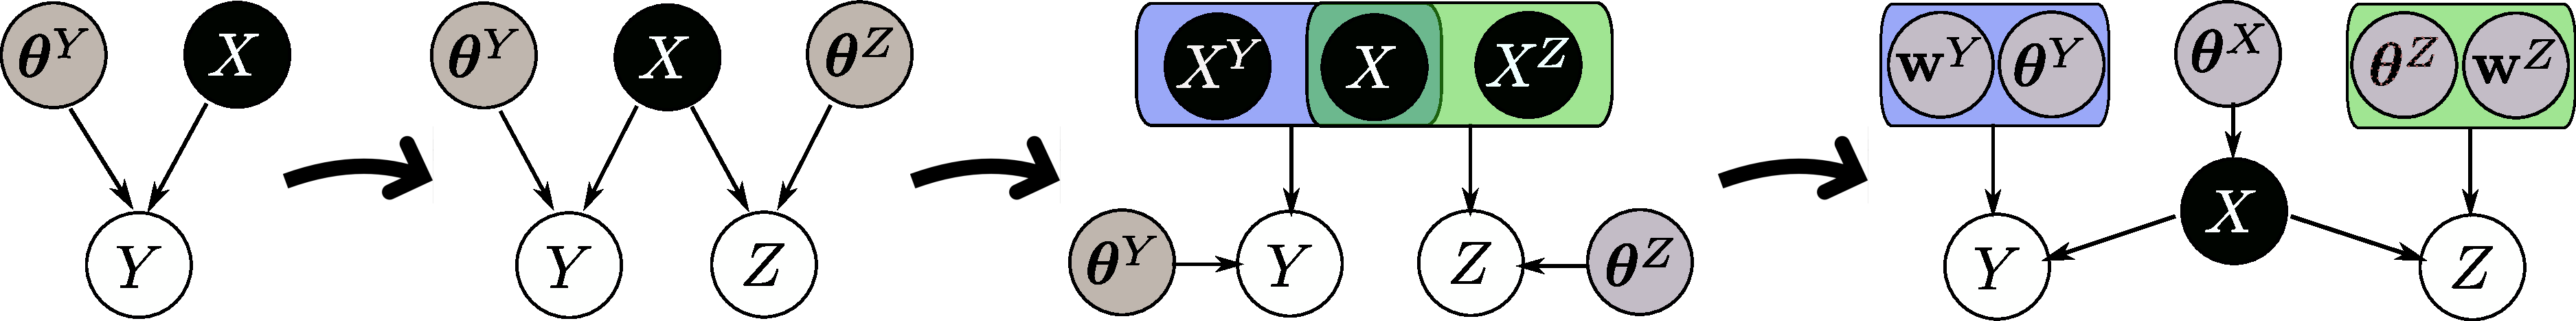
\includegraphics[width=0.7\textwidth]{../diagrams/graphicalmodel.pdf}
  \end{center}
 % \vspace{-8pt}
  \caption{ %\small {\it
    Evolution of the structure of GP-LVM model variants. \emph{Far left:}
    \citet{Lawrence:2005vk}'s original model is shown, a single latent
    variable $X$ is used to represent the observed data $Y$. Evolved
    shared models then (\emph{left} to \emph{right}) assume firstly,
    that all of the variance in the observations was shared \cite{Shon:2006wr}. Secondly, \citet{Ek:2008up} introduced private latent spaces to explain variance specific to one of the views. MAP estimates used in this model meant the structure of the latent space could not be automatically determined. The rightmost image shows the model we propose in this
    paper.
%
%Here, the kernel hyperparameters are actually $\bftheta^{\{Y,Z\}} = \{ \sigma_{ard}^{ \{Y,Z\} }, \bfw^{\{Y,Z\}} \}$,
%but in the figure we explicitly used $\bfw^{\{Y,Z\}}$, to emphasize the usage of ARD covariance functions.    
%
     In this figure we have separated the ARD weights $\bfw^{\{Y,Z\}}$ from the full set of model hyperparameters
      $\bftheta^{\{Y,Z\}} = \{ \sigma_{\epsilon}^{\{Y,Z\}}, \sigma_{ard}^{\{Y,Z\}}, \bfw^{\{Y,Z\}} \}$, 
      just to emphasize the usage of ARD covariance functions.
 %   
     The latent space $X$ is marginalised out and we learn a
    distribution of latent points for which additional hyperparamters
    encode the relevance of each dimension independently for the
    observation spaces and, thus, automatically define a factorisation
    of the data. The distribution $p(X) = p(X|\bftheta^X)$ placed on the latent space also enables the incorporation of prior knowledge about its structure.
      %By
      %introducing additional hyperparameters to the model encoding the
      %relevance of each dimension independently for the observation
      %spaces we can automatically learn the factorization of the data.
 % }
  }
 \label{fig:grModel}
\end{figure*}
We wish to recover a factorized latent representation such that the
variance shared between different observation spaces can be aligned
and separated from variance that is specific (private) to the separate
views.  In manifold relevance determination the notion of a hard
separation between private and shared spaces is relaxed to a
continuous setting. The model is allowed to (and indeed often does)
completely allocate a latent dimension to private or shared spaces,
but may also choose to endow a shared latent dimension with more or
less relevance for a particular data-view. Importantly, this
factorization is learned from data by maximizing a variational lower
bound on the model evidence, rather than through construction of
bespoke regularizers to achieve the same
effect.  
%
The model we propose can be seen as a generalisation of the traditional
approach to manifold learning; we still
assume the existence of a low-dimensional representation encoding the
underlying phenomenon, but the variance contained in an observation
space does not necessarily need to be governed by the full manifold,
as traditionally assumed, nor by a subspace geometrically orthogonal
to that, as assumed in \citet{Salzmann:2010vh}.
%
% What makes this possible is the
% marginalisation of the latent space $X$.  Without this the likelihood
% would always increase by the use of additional latent dimensions,
% since the number of model parameters increases proportionally to $Q$,
% and the ARD weights would be unable to ``switch off'' dimensions that
% are irrelevant for a specific observation space.

%%  to individually 
%% the relevance of each latent dimension therefore selecting a
%% ``smooth'' subspace of the manifold 

%%  allowing each generative mapping to separately determine the
%% relevance of each latent dimension.
%% %This allows us to learn a
%% %factorized latent space where a dimension considered important, as
%% %indicated by the ARD weight, by more than one observation space is
%% %considered shared and a dimension considered important by a single
%% %space as private.  
%% %
%% This means that we automatically learn a ``soft'' factorization
%% of the latent space without having to rely on hand crafted
%% regularizers such as in \cite{Salzmann:2010vh}. 
%% %
%% What makes this possible is the marginalisation of the latent space
%% $X$.  Without this the likelihood would always increase by the use of
%% additional latent dimensions, since the number of model parameters
%% increases proportionally to $Q$, and the ARD weights would be unable
%% to ``switch off'' dimensions that are irrelevant for a specific
%% observation space.


%
%%% There is some redundancy here...
%
%The traditional approach to manifold learning has been to assume
%that the observed high-dimensional data have been generated from a
%low-dimensional latent variable. The model we propose  %in this paper
%can be seen as a generalisation of this, as we still
%
%
The expressive power of our model comes from the ability to consider
non-linear mappings within a Bayesian framework.  Specifically, our
$D_Y$ latent functions $f^Y_d$ are selected to be independent draws of
a zero-mean GP with an ARD covariance function of the form:
\begin{align}
  k^Y \left( \bfx_i, \bfx_j \right) = {} & (\sigma_{ard}^Y)^2 e^{ -
    \frac{1}{2} \sum_{q=1}^{Q} w^Y_q \left( x_{i,q} - x_{j,q} \right)
    ^2 },
\label{ARDkernel}
\end{align}
and similarly for $f^Z$. Accordingly, we can learn a common latent
space\footnote{As we will see in the next section, we actually learn a
  common \emph{distribution} of latent points.}
%, giving us a set of  latent points (mean of the distribution) and associated variance.}
but we allow the two sets of ARD weights $\bfw^Y = \{ w_q^Y
\}_{q=1}^Q$ and $\bfw^Z = \{ w_q^Z \}_{q=1}^Q$ to automatically infer
the responsibility of each latent dimension for generating points in
the $Y$ and $Z$ spaces respectively.  We can then automatically
recover a segmentation of the latent space $X = \left( X^Y, X^s, X^Z
\right)$, where $X^s \in \mathbb{R}^{N \times Q_s}$ is the shared
subspace, defined by the set of dimensions $q \in [1, ... ,Q]$ for
which $w^Y_q, w^Z_q > \delta$, with $\delta$ being a number close
to zero and $Q_s \leq Q$. This equips the model with further
flexibility, because it allows for a ``softly'' shared latent space,
if the two sets of weights are both greater than $\delta$ but
dissimilar, in general.  As for the two private spaces, $X^Y$ and
$X^Z$, they are also being inferred automatically along with their
dimensionalities $Q_Y$ and $Q_Z$ \footnote{In general, there will also
  be dimensions of the initial latent space which are considered
  unnecessary by both sets of weights. 
  %If the subspace
  %corresponding to these irrelevant latent dimensions is denoted with
  %$X^U$, then the actual factorisation can be written more precisely
  %as $X = \left( X^Y, X^s, X^Z, X^U \right)$.
  }.
%
More precisely:
\begin{equation}
  X^Y = \{ \bfx_q \}_{q=1}^{Q_Y}: \bfx_q \in X, \; w^Y_q > \delta, \;  w^Z_q < \delta
\end{equation}
and analogously for $X^Z$. Here, $\bfx_q$ denotes columns of $X$,
while we assume that data are stored by rows.  All of the above are
summarised in the graphical model of figure \ref{fig:grModel}.
%


\subsection{Bayesian training}
\par 
%From the previous section it follows that the model hyperparameters
%are $\bftheta = \{ \sigma_{\epsilon}^{\{Y,Z\}}, \sigma_{ard}^{\{Y,Z\}}, \bfw^{\{Y,Z\}} \}$.
The fully Bayesian training procedure requires maximisation of
the logarithm of the joint \emph{marginal} likelihood $p(Y,Z |
\bftheta) = \int p(Y,Z | X, \bftheta) p(X) \intd X$, where a prior
distribution is placed on $X$. This prior may be a standard normal distribution or may generally depend on a set
of parameters $\bftheta^X$. By
looking again at \eqref{eq:likelihood} we see that the above integral is
intractable due to the nonlinear way in which $X$ appears in
$p(F^{\{Y,Z\}}|X,\bftheta^{\{Y,Z\}})$. Standard variational approximations
are also intractable in this situation. Here, we describe a non-standard
method which leads to an analytic solution.

%Similarly to standard mean field approximations, we start by seeking to maximise
As a starting point, we consider the mean field methodology and seek to maximise
a variational lower bound $F_v(q,\bftheta)$ on the logarithm of the
true marginal likelihood by relying on a variational distribution which factorises as
$q(\Theta)q(X)$, where we assume that $q(X)
\sim \mathcal{N}(\bfmu, S)$. 
%As will be explained later more clearly, in our approach 
As will be explained later more clearly, in our approach $q(\Theta)$ is a distribution which depends on additional
variational parameters $\Theta=\{\Theta^Y, \Theta^Z\}$ so that $q(\Theta) = q(\Theta^Y) q(\Theta^Z)$.
These additional parameters $\Theta$ as well as the exact form of $q(\Theta)$
will be defined later on, as they constitute the most crucial ingredient of our non-standard variational approach.
%$ = q(\Theta^Y)q(\Theta^Z)$ is a 
% and $q(\Theta)$ depends on additional variational
%parameters $\Theta$ and will be defined later on,
%as its form is the main ingredient of our non-standard variational
%approach.

  By dropping the model hyperparameters $\bftheta$ from our expressions, 
  for simplicity, we can use Jensen's inequality and obtain a variational
bound $F_v(q) \leq \log p(Y,Z)$:
\begin{align}
F_v(q) & = \int q(\Theta) q(X) \log \left( \frac{p(Y|X)p(Z|X)}{q(\Theta)}\frac{p(X)}{q(X)} \right) \intd X \nonumber \\
      % & = \int q(\Theta) q(X) \log \frac{p(Y,Z|X)}{q(\Theta)} \intd X - \int \cancel{q(\Theta)} q(X) \log \frac{q(X)}{p(X)} \intd X
      & = \mathcal{L}_Y + \mathcal{L}_Z - \text{KL} \left[ q(X) \parallel p(X)\right], \label{eq:bound}
\end{align}
where % we introduced the additional factorisation $q(\Theta)=q(\Theta^Y)q(\Theta^Z)$ so that
$\mathcal{L}_Y = \int q(\Theta^Y) q(X) \log
\frac{p(Y|X)}{q(\Theta^Y)} \intd X$ and similarly for $\mathcal{L}_Z$.
However, this does not solve the problem of intractability since the
challenging terms still appear in $\mathcal{L}_Y$ and $\mathcal{L}_Z$.
To circumvent this problem, we follow \citet{Titsias:bayesGPLVM10} and
apply the ``data augmentation'' principle, \ie we expand the joint
probability space with $M$ extra samples $U^Y$ and $U^Z$ of the latent
functions $f^Y$ and $f^Z$ evaluated at a set of pseudo-inputs (known
as ``inducing points'') $\bar{X}^Y$ and $\bar{X}^Z$
respectively. Here, $U^Y \in \mathbb{R}^{M_Y \times D_Y}$, $U^Z \in
\mathbb{R}^{M_Z \times D_Z}$, $\bar{X}^Y \in \mathbb{R}^{M_Y \times
  Q}$, $\bar{X}^Z \in \mathbb{R}^{M_Z \times Q}$ and $M = M_Y+M_Z$.
The expression of the joint probability is as before except for the
term $p(Y|X)$ which now becomes:
 \begin{align}
  p(Y|X, \bar{X}^Y) = \int & p(Y|F^Y)p(F^Y|U^Y,X, \bar{X}^Y) \cdot \nonumber \\
  				           & p(U^Y|\bar{X}^Y) \intd F^Y \intd U^Y \label{eq:pYXXbar}
  \end{align}
%
and similarly for $p(Z|X)$. 
The integrations over $U^{\{Y,Z\}}$ are tractable if we assume 
Gaussian prior distributions for these variables.
%
As we shall see, the inducing points are \emph{variational} rather than
model parameters.  More details on the variational learning of
inducing variables in GPs can be found in
\citet{Titsias:variational09}.
%
\par Analogously to \citet{Titsias:bayesGPLVM10}, we are now able to
define $q(\Theta) =  q(\Theta^Y) q(\Theta^Z) $ as
\begin{equation}
\label{qTheta}
q(\Theta) = \prod_{\mathcal{K}=\{Y,Z\}} q(U^\mathcal{K}) p(F^\mathcal{K}|U^\mathcal{K},X,\bar{X}^\mathcal{K}),
\end{equation} 
where $q(U^{\{Y,Z\}})$ are free form distributions.  In that way, the
$p(F^\mathcal{K}|U^\mathcal{K},X,\bar{X}^\mathcal{K})$ factors cancel
out with the ``difficult'' terms of $\mathcal{L}_Y $ and
$\mathcal{L}_Z$, as can be seen by replacing equations \eqref{qTheta}
and \eqref{eq:pYXXbar} back to \eqref{eq:bound}, which now becomes our
final objective function and can be trivially extended for more than
two observed datasets. This function is jointly maximised with respect
to the model parameters, involving the latent space weights $\bfw^Y$
and $\bfw^Z$, and the variational parameters $\{\bfmu, S,
\bar{X}\}$. As in standard variational inference, this optimisation
gives, as a by-product, an approximation of $p(X|Y,Z)$ by $q(X)$, \ie
we obtain a distribution over the latent space. This adds extra
robustness to our model, since previous approaches rely on MAP
estimates for the latent points. More detailed derivation of the
variational bound can be found in the suppl.\ material.


%\subsection{Dynamical Modelling}
\noindent{\bf Dynamical Modelling:}
The model formulation described previously is also
covering the case when we wish to additionally model correlations
between datapoints of the same output space, \eg when $Y$ and $Z$ are
multivariate timeseries. For the dynamical scenario we follow
\citet{Damianou:vgpds11,Lawrence:hgplvm07} and choose the prior on the
latent space to depend on the observation times $\bft \in \mathbb{R}^N$, \eg a GP with a covariance function $k =
k(t,t^\prime)$. With this approach, we are also allowed to learn the
structure of multiple independent sequences which share some commonality by
learning a common latent space for all timeseries while, at the same
time, ignoring correlations between datapoints belonging to
different sequences.





%\subsection{Inference \label{inference}}
\noindent{\bf Inference:}
Given a model which is trained to jointly represent two output spaces
$Y$ and $Z$ with a common but factorised input space $X$, we wish to
generate a new (or infer a training) set of outputs $Z^* \in
\mathbb{R}^{N^* \times D_Z}$ given a set of (potentially partially)
observed test points $Y^* \in \mathbb{R}^{N^* \times D_Y}$.  This is
done in three steps. Firstly, we predict the set of latent points $X^*
\in \mathbb{R}^{N^* \times Q}$ which is most likely to have generated
$Y^*$. For this, we use an approximation to the posterior
$p(X^*|Y^*,Y)$, which has the same form as for the standard Bayesian
GP-LVM model \cite{Titsias:bayesGPLVM10} and is given by a variational
distribution $q(X,X^*)$. To find $q(X,X^*)$ we optimise a variational
lower bound on the marginal likelihood $p(Y,Y^*)$ which has analogous
form with the training objective function
\eqref{eq:bound}. Specifically, we ignore $Z$ and replace $Y$ with
$(Y,Y^*)$ and $X$ with $(X,X^*)$ in \eqref{eq:bound}.
%similar to the variational distribution $q(X)$ learned during training.
In the second step, we find the training latent points $X_{NN}$ which
are closest to $X^*$ in the \emph{shared} latent space.  In the third
step, we find outputs $Z$ from the likelihood $p(Z | X_{NN})$.  This
procedure returns the set of training points $Z$ which best match the
observed test points $Y^*$.  If we wish to generate novel outputs, we
have to propagate the information recovered when predicting $X^*$.
Since the shared latent space encodes the same kind of information for
both datasets, we can achieve the above by simply replacing the
features of $X_{NN}$ corresponding to the shared latent space, with
those of $X^*$.
%
 % A simple way of doing this is to replace the features of $X_{NN}$
 % corresponding to the shared latent space, with those of $X^*$.
 % This is a reasonable idea, since the shared latent space encodes
 % the same kind of information for both datasets.


% A slightly more sophisticated approach is to also exploit the
% continuous nature of the optimised weights $\bfw_Y$ and give less
% importance to the dimensions of $X^*$ for which $w_Y^q$ is small,
% because these features are predicted with large uncertainty
% (variance).  For example, we can create a new set of latent points
% $\hat{X}^{*}$ so that its private dimensions match those of $X_{NN}$
% and its shared dimensions are found by averaging the shared
% dimensions of $X^*$ and $X_{NN}$ as appropriate based on
% $\bfw_Y$. We can then generate outputs from $p(Z^* | \hat{X}^{*})$.


%\subsection{Complexity}
\noindent{\bf Complexity:}
As in common sparse methods in Gaussian processes
\cite{Titsias:variational09}, the typical cubic complexity reduces to
$O(NM^2)$, where $N$ and $M$ is the total number of training and
inducing points respectively. 
In our experiments we set $M=100$.
 Further, the model scales only
linearly with the data dimensionality. Indeed, the Gaussian densities
in equation \eqref{eq:bound} result in an objective function which
only involves the data matrices $Y$ and $Z$ in expressions of the form
$Y Y^\T$ and $Z Z^\T$ which are $N \times N$ matrices no matter how
many features $D_Y$ and $D_Z$ are used to describe the original
data. Also, these quantities are constant and can be
precomputed. Consequently, our approach can model datasets with
very large numbers of features.


%%% Local Variables: 
%%% mode: latex
%%% TeX-master: "../svargplvmICML2012"
%%% End: 
